\chapter{Data Preparation}
\label{chap:dataPrep}

The Data Preparation utility allows exploring the distribution of the data in the
selected Data File and the impact that different Data Preparation options have over
the data.

\section{The interface}

The Data Preparation tab is divided in two main regions (\autoref{fig:dataPrepTab}).

\begin{figure}[h]
    \centering
    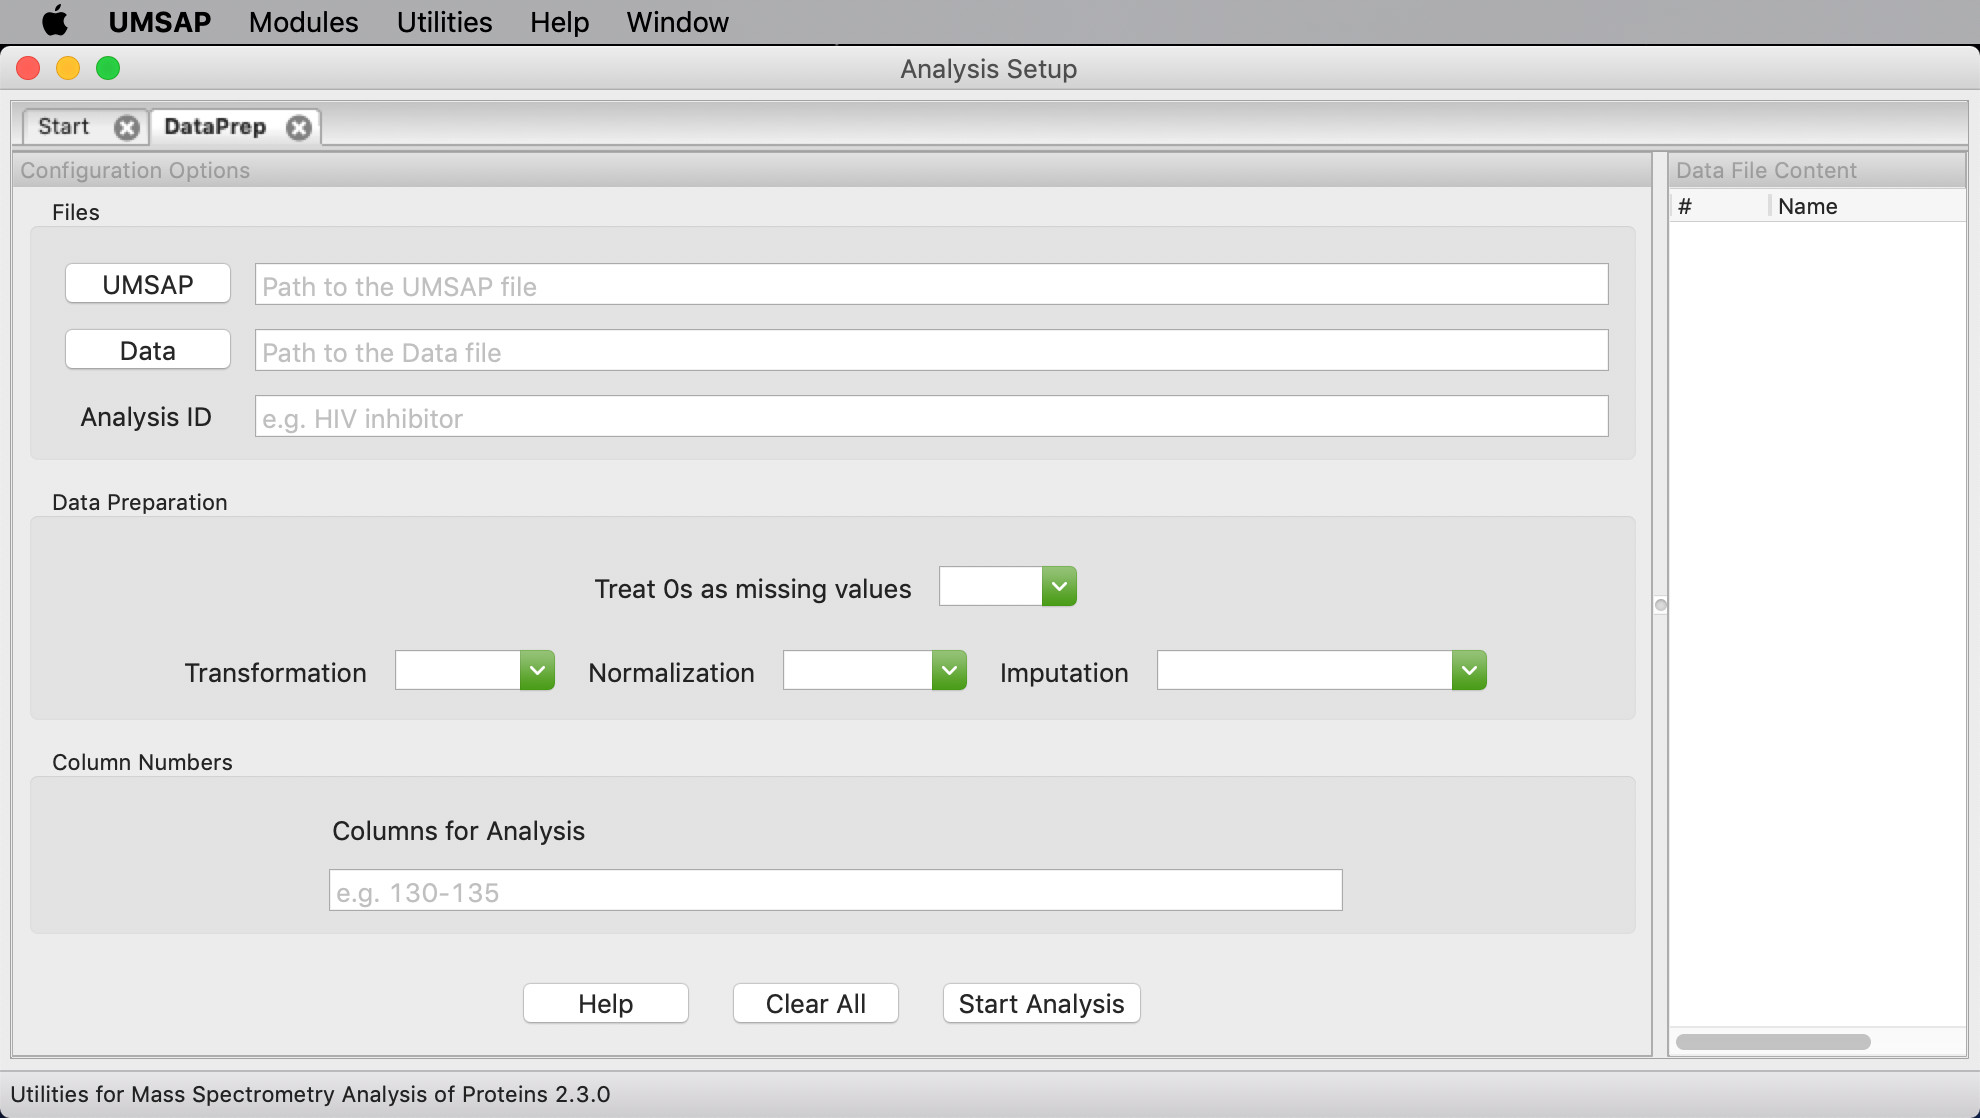
\includegraphics[width=0.7\textwidth]{./IMAGES/DATAPREP/DataPrep.jpg}
    \caption[The Data Preparation tab]{\textbf{The Data Preparation tab.}
    This tab allows to perform a statistical exploration of the data contained in
    a given Data file.} 
    \label{fig:dataPrepTab}
    \vspace{-5pt}
\end{figure}

The Data File Content region holds only a list to show the name of the columns in
the selected Data File. The list will be automatically filled after selecting the
file.

The Configuration Options region contains all the fields needed to configure and
run the analysis. 

Section Files contains two buttons and a text field. Here users select the input
and output files for the analysis.

\num{1}. The button UMSAP allows users to browse the file system to select the location
and name of the .umsap file. When selecting an already existing .umsap file the operating
system will ask if it is ok to replace the file, the answer can be yes since UMSAP
will never overwrite or replace an .umsap file, instead the new analysis will be
added to the already existing file. Only .umsap files can be selected here.

\num{2}. The button Data allows users to browse the file system to select the input
data file that will be used for the analysis. The Data file is expected to be a
plain text file with tab separated columns and the name of the columns in the first
row of the file. In addition, columns to be analyzed must contain only numbers and
must be of the same length. Only .txt files can be selected here.

\num{3}. The text field Analysis ID allows users to provide an ID for the analysis
to be run. The date and time of the analysis will be automatically added to the
beginning of the name.

Section Data Preparation contains four dropdown boxes. Here users select how the data
in the Data file should be prepared before starting an analysis.

\num{1}. The dropdown Treat \num{0}s as missing values allows user to define how
to handle \num{0} values present in the Data file.

\num{2}. The dropdown Transformation allows user to select the Transformation method
to be applied to the data.

\num{3}. The dropdown Normalization allows users to select the Normalization method
to be applied to the data.

\num{4}. The dropdown Imputation allows user to select the Imputation method used
to replace missing values in the data.

Section Column numbers contains a text field. Here users specify the Columns in the
Data File to be used during the Data Preparation steps. Only integers can be accepted
here. Column numbers can be copied (Cmd+C) and paste (Cmd+P) from the selected rows
in the list on region Data File Content.

The bottom of the region contains three buttons.

\num{1}. The button Help leads to an online tutorial about Correlation Analysis in
UMSAP.

\num{2}. The button Clear All will delete all user input from the tab.

\num{3}. The button Start Analysis starts the Correlation Analysis.

\section{The analysis}